\documentclass{beamer}
\usepackage[english,russian]{babel}
\usepackage[utf8]{inputenc}
\usepackage{amsmath}
\usepackage{hyperref}
\usetheme{Warsaw}
\usepackage{listings}
\usepackage{xcolor}
\usepackage{tikz}
\usetikzlibrary{graphs}
\usepackage{algpseudocode}

\lstset{
    frame=tb,
    tabsize=4,
    showstringspaces=false,
    numbers=left,
    commentstyle=\color{green},
    keywordstyle=\color{blue},
    stringstyle=\color{red},
    emph={baz},
    emphstyle=\textbf
}

\begin{document}

\title{Задачи разрешимости логических формул и приложения\newline Лекция 10. Формулы с кванторами}
\author{Роман Холин}
\institute{Московский государственный университет}
\date{Москва, 2022}

\begin{frame}
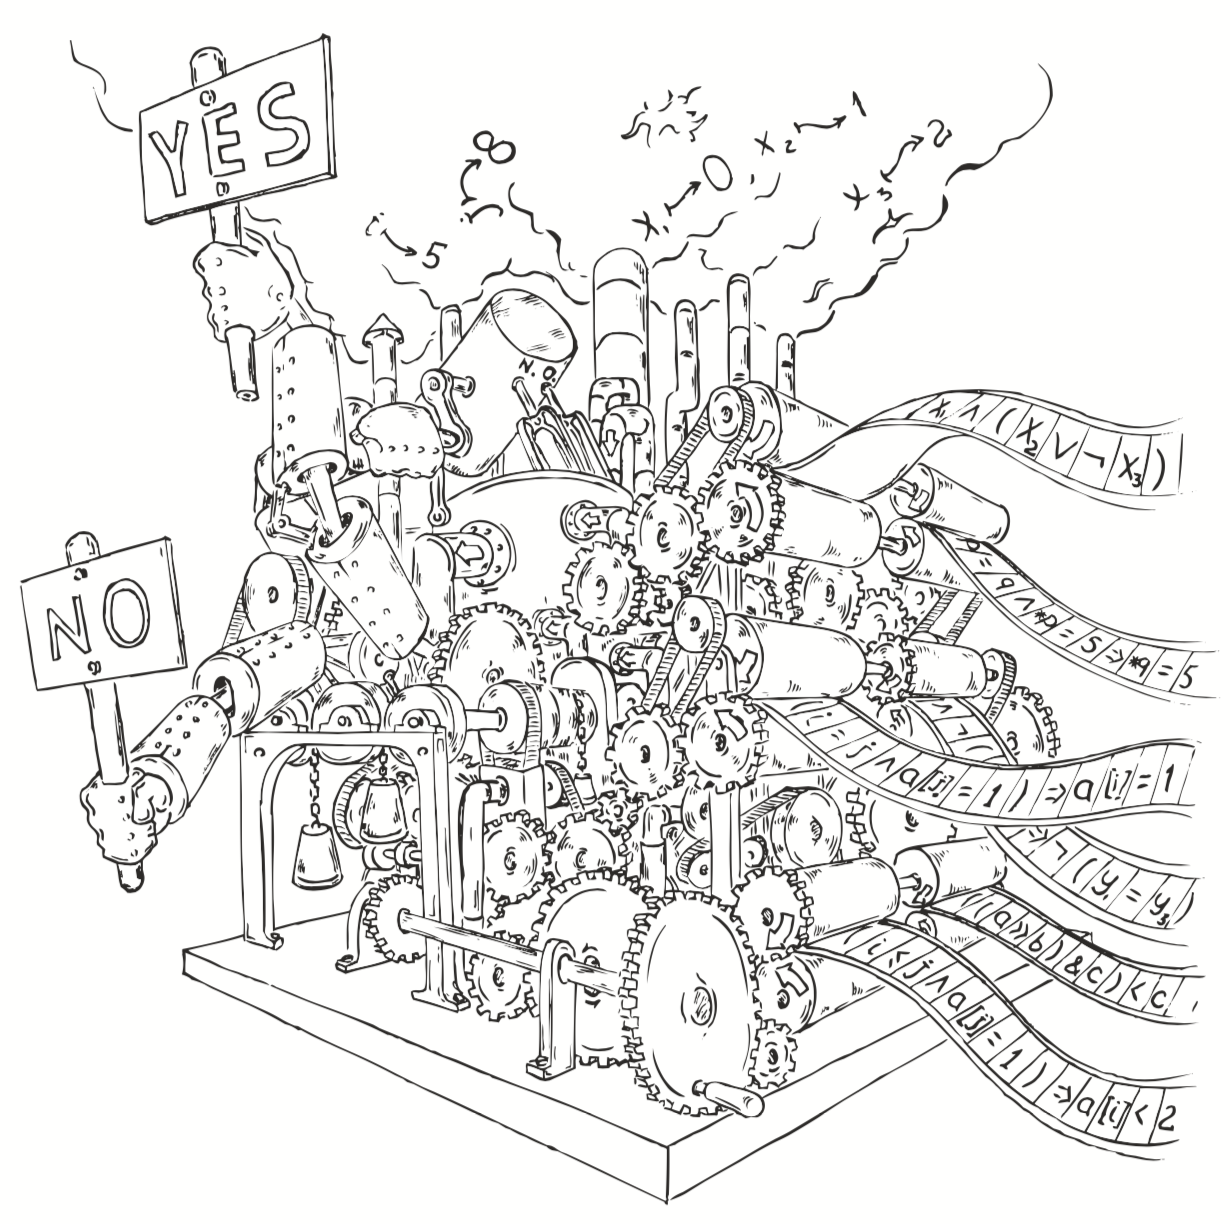
\includegraphics[scale=0.5]{../decision-procedure.png}
\end{frame}

\frame{\titlepage}

\begin{frame}{Определения}
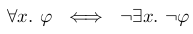
\includegraphics[scale=0.5]{all_and_exist.png}\newline
\end{frame}

\begin{frame}{Определения}
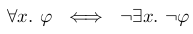
\includegraphics[scale=0.5]{all_and_exist.png}\newline
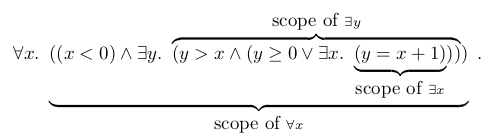
\includegraphics[scale=0.5]{scope.png}\newline
\end{frame}

\begin{frame}{Определения}
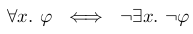
\includegraphics[scale=0.5]{all_and_exist.png}\newline
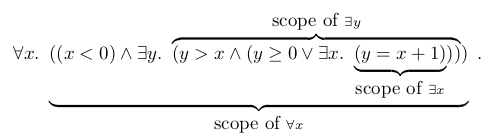
\includegraphics[scale=0.5]{scope.png}\newline
\begin{itemize}
\item Переменная называется свободной, если она не привязана к квантору
\end{itemize}
\end{frame}

\begin{frame}{Определения}
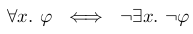
\includegraphics[scale=0.5]{all_and_exist.png}\newline
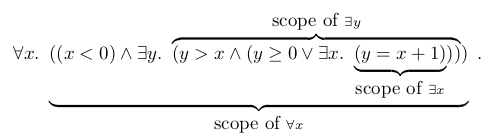
\includegraphics[scale=0.5]{scope.png}\newline
\begin{itemize}
\item Переменная называется свободной, если она не привязана к квантору
\item Формула замкнута, если не содержит свобожных переменных
\end{itemize}
\end{frame}

\begin{frame}{QBF}
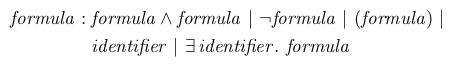
\includegraphics[scale=0.5]{qbf.png}\newline
\end{frame}

\begin{frame}{QBF}
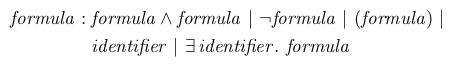
\includegraphics[scale=0.5]{qbf.png}\newline
Сложность - PSPACE
\end{frame}

\begin{frame}{QDLA}
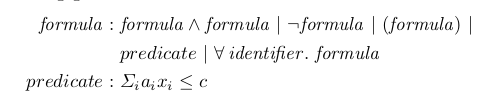
\includegraphics[scale=0.5]{qdla.png}\newline
\end{frame}

\begin{frame}{Пренексная нормальная форма}
\begin{itemize}
\item Формула находится в Пренексной нормальной форме, если она имеет форму $Q[n]V[n]\dots Q[1]V[1].<quantifier-free formula>$,
где $Q[i]$ - квантор, $V[i]$ - переменная
\end{itemize}
\end{frame}

\begin{frame}{Пренексная нормальная форма}
\begin{itemize}
\item Формула находится в Пренексной нормальной форме, если она имеет форму $Q[n]V[n]\dots Q[1]V[1].<quantifier-free formula>$,
где $Q[i]$ - квантор, $V[i]$ - переменная
\item Для каждой кванторной формулы существует эквивалентная ей формула в пренексной нормальной форме
\end{itemize}
\end{frame}

\begin{frame}
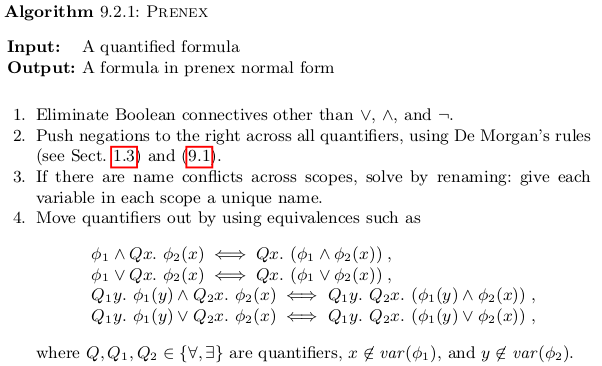
\includegraphics[scale=0.5]{prenex.png}\newline
\end{frame}

\begin{frame}{Пример}
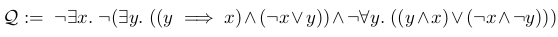
\includegraphics[scale=0.5]{prenex_example.png}\newline
\end{frame}

\begin{frame}{Проекция}
Проекция формулы $Q[n]V[n]\dots Q[2]V[2].\exists x.\phi$\newline
называют формулу $Q[n]V[n]\dots Q[2]V[2].\phi$
\end{frame}

\begin{frame}{Пример}
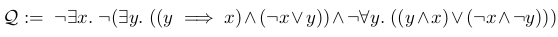
\includegraphics[scale=0.5]{prenex_example.png}\newline
\end{frame}

\begin{frame}
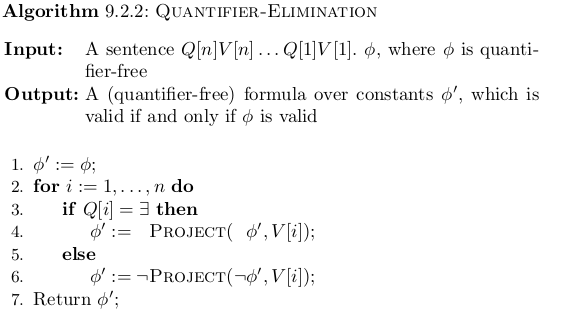
\includegraphics[scale=0.5]{quantifier-elimination.png}\newline
\end{frame}

\begin{frame}{Элиминация кванторов для QBF}
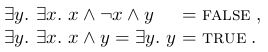
\includegraphics[scale=0.5]{elem_qbf1.png}\newline
\end{frame}

\begin{frame}{Элиминация кванторов для QBF}
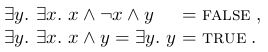
\includegraphics[scale=0.5]{elem_qbf1.png}\newline
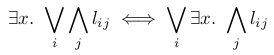
\includegraphics[scale=0.5]{elem_qbf2.png}\newline
\end{frame}

\begin{frame}{Проекция с помощью бинарной резолюции}
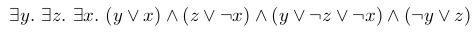
\includegraphics[scale=0.5]{reduction1.png}\newline
\end{frame}

\begin{frame}{Проекция с помощью бинарной резолюции}
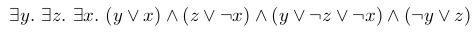
\includegraphics[scale=0.5]{reduction1.png}\newline
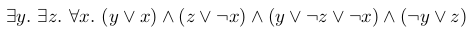
\includegraphics[scale=0.5]{reduction2.png}\newline
\end{frame}

\begin{frame}{Пример}
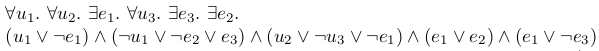
\includegraphics[scale=0.5]{reduction_ex.png}\newline
\end{frame}

\begin{frame}{Элиминация кванторов с помощью расширения Шенона}
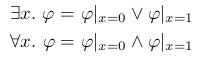
\includegraphics[scale=0.5]{expansion_based.png}\newline
\end{frame}

\begin{frame}{Пример}
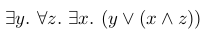
\includegraphics[scale=0.5]{expansion_based_ex.png}\newline
\end{frame}

\begin{frame}{Элиминация кванторов для QDLA}
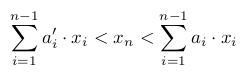
\includegraphics[scale=0.5]{linear1.png}\newline
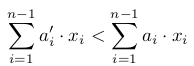
\includegraphics[scale=0.5]{linear2.png}\newline
\end{frame}

\begin{frame}{Пример}
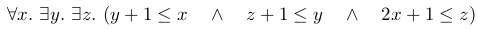
\includegraphics[scale=0.5]{linear_ex.png}\newline
\end{frame}

\begin{frame}{Наивный алгоритм разрешения QBF}
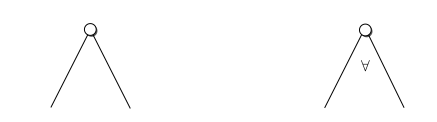
\includegraphics[scale=0.5]{cdcl1.png}\newline
\end{frame}

\begin{frame}{Наивный алгоритм разрешения QBF}
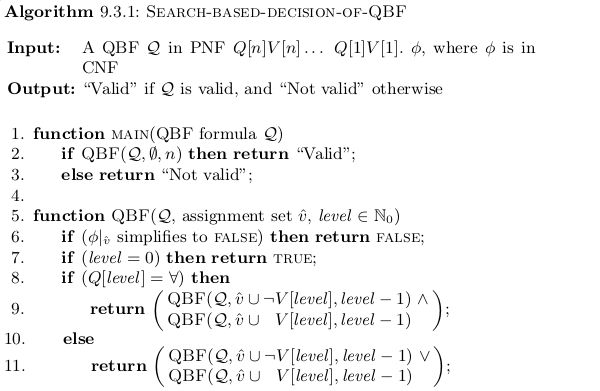
\includegraphics[scale=0.5]{cdcl2.png}\newline
\end{frame}

\begin{frame}
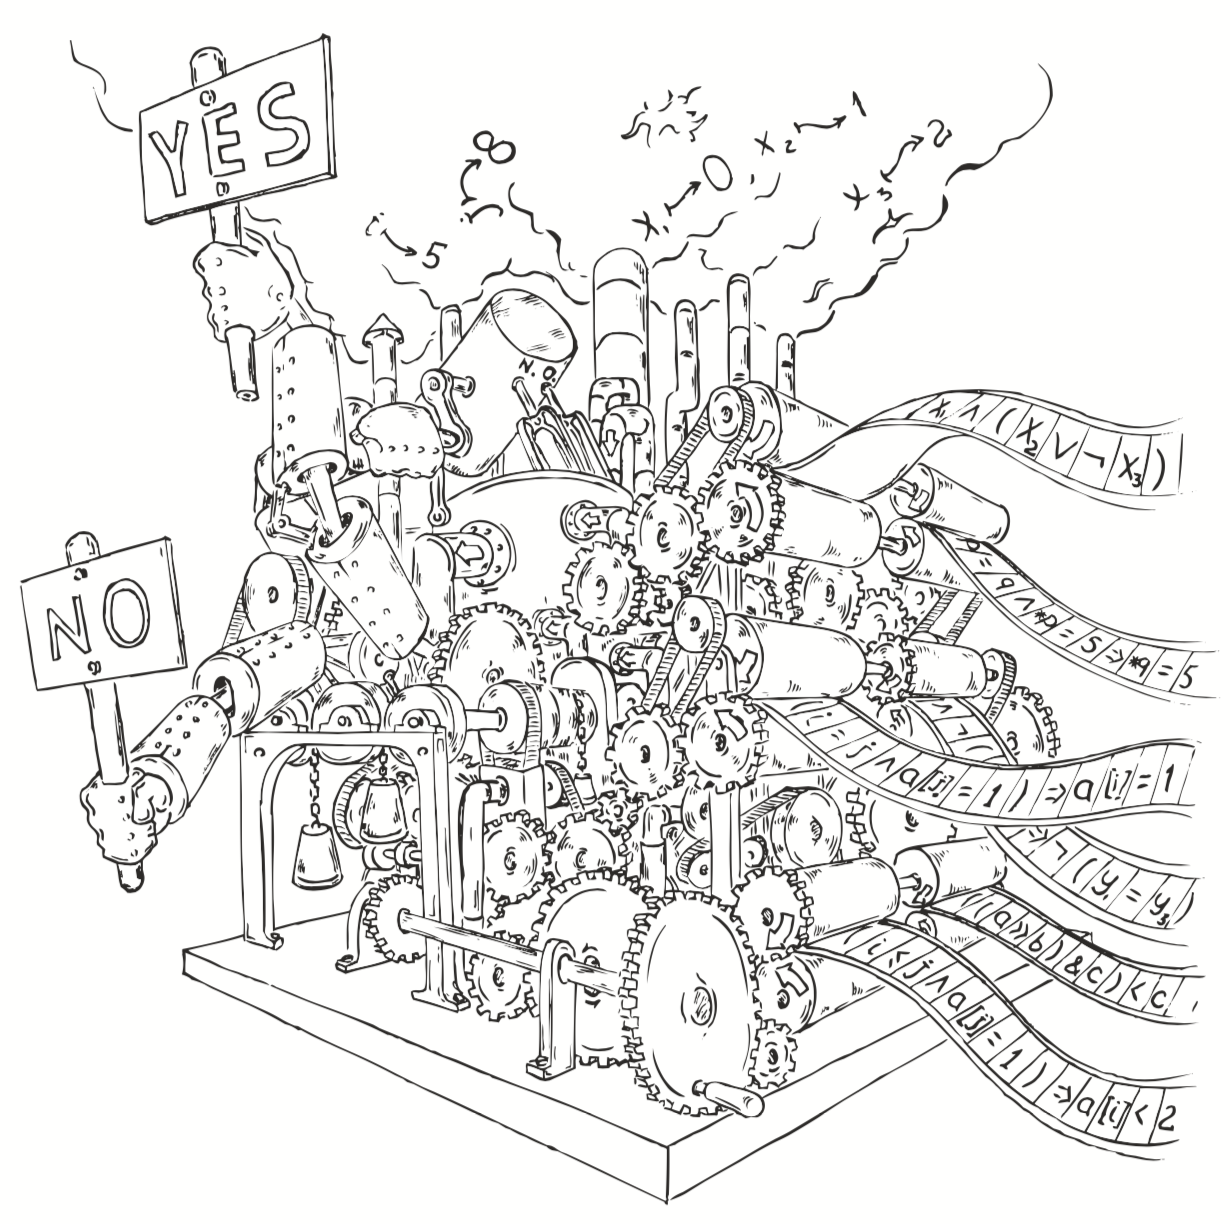
\includegraphics[scale=0.5]{../decision-procedure.png}
\end{frame}

\end{document}
